% !TEX program = xelatex
\let\nofiles\relax
\documentclass{article}
\usepackage{graphicx}
\usepackage{setspace}
% \usepackage{ctex}
\usepackage{indentfirst}
\setlength{\parindent}{2em}  % 用于首行缩进

\usepackage{bm}
\usepackage{amsmath}
\usepackage{mathtools}
\usepackage{caption}
\usepackage{subfigure}
\usepackage{amssymb}
\usepackage{amsthm} % 使用定理环境
% \usepackage{ntheorem}

\usepackage{multirow}
\usepackage{pdfpages}
\usepackage{cite}   % 文献
\usepackage[colorlinks,linkcolor=red,anchorcolor=blue,citecolor=green,CJKbookmarks=True]{hyperref}  % 使用链接 但不用默认属性
% CJKbookmarks让链接支持中文
% \usepackage{hyperref}
% \usepackage{geometry}
% \geometry{a4paper,scale=0.8}

\usepackage{geometry}
\geometry{a4paper,left=1in,right=1in,top =1in, bottom = 1in}
\setstretch{1.5}   %  改变行间距
% \newgeometry{left = 2 cm, top= 3 cm}

\title{Seat Planning and Assignment with Social Distancing}
% \author{Dis$\cdot$ count}

% \newtheorem{algorithm}{Algorithm}
\usepackage[linesnumbered,tworuled]{algorithm2e}
\SetKwComment{Comment}{/* }{ */}
\RestyleAlgo{ruled}

\newtheorem{thm}{\hspace{2em}Theorem}
\newtheorem{lem}{\hspace{2em}Lemma}
\newtheorem*{pf}{}
\newtheorem{remark}{\hspace{2em}Remark}
\newtheorem{corollary}{\hspace{2em}Corollary}
\newtheorem{prop}{\hspace{2em}Proposition}
\newtheorem{definition}{Definition}
\newtheorem{example}{Example}
\DeclareMathOperator{\sign}{sign}
% \newcommand{\sign}{\text{sign}}
\newcommand{\X}{\mathbf{X}}


\begin{document}
\maketitle{}

% !TEX root = sum1.tex

\section*{Abstract}



Keywords: Social Distancing, Seat Assignment, Dynamic Arrival.


% !TEX root = sum1.tex
\section{Introduction}
Social distancing has been a proven concept to contain the spread of an infectious disease. As a general principle, social distancing can be implemented in various forms. The basic requirement of social distancing is the specification of a minimum physical distance between people in public areas. For example, the World Health Organization suggests social distancing by ``keep physical distance of at least 1 meter from others'' (https://www.who.int/emergencies/diseases/novel-coronavirus-2019/advice-for-public). In the US, the CDC refers to social distancing as ``keeping a safe space between yourself and other people who are not from your household.'' (https://stacks.cdc.gov/view/cdc/90522)

Note that under such a requirement, social distancing is actually applied with respect to groups of people. In Hong Kong, the government has adopted social distancing measures, in the recent Covid 19 pandemic, by limiting the size of groups in public gathering to two, four, and six people per group over time. Moreover, the Hong Kong government has also adopted the limit of the total number of people in a venue; for example, restaurants can operate at 50\% or 75\% of their normal seating capacity.


While the above practice of social distancing has been recognized for its primary function,  it is not clear how the entire economy will be affected. This is an important issue in the service sector where social distancing implies fewer clients and lower revenue. The situation is especially complicated under multiple social distancing measures, such as physical distance between groups, limit on the size of groups, and the occupancy rate of the venue. This naturally raises questions regarding the relationship of these measures, e.g., which is relatively more effective under different conditions, whether they compliment or contradict with each other, and more importantly, is it possible to align these measures so that they can be implemented coherently? 

We will address the above issues of social distancing in the context of seating arrangement in a venue, such as a cinema or a conference hall. The venue is equipped with seats of multiple rows.  People come in groups where each group of people will sit consecutively in one row. The social distancing requirement.


% Governments worldwide have been faced with the challenge of reducing the spread of Covid-19 while minimizing the economic impact. Social distancing has been widely implemented as the most effective non-pharmaceutical treatment to reduce the health effects of the virus. 
% This website records a timeline of Covid-19 and the relevant epidemic prevention measures\cite{Covid19Timeline}. For instance, in March 2020, the Hong Kong government implemented restrictive measures such as banning indoor and outdoor gatherings of more than four people, requiring restaurants to operate at half capacity. As the epidemic worsened, the government tightened measures by limiting public gatherings to two people per group in July 2020. As the epidemic subsided, the Hong Kong government gradually relaxed social distancing restrictions, allowing public group gatherings of up to four people in September 2020. In October 2020, pubs were allowed to serve up to four people per table, and restaurants could serve up to six people per table. Specifically, the Hong Kong government also implemented different measures in different venues \cite{Gov202209}. For example, the catering businesses will have different social distancing requirements depending on their mode of operation for dine-in services. They can operate at 50\%, 75\%, or 100\% of their normal seating capacity at any one time, with a maximum of 2, 2, or 4 people per table, respectively. Bars and pubs may open with a maximum of 6 persons per table and a total number of patrons capped at 75\% of their capacity. The restrictions on the number of persons allowed in premises such as cinemas, performance venues, museums, event premises, and religious premises will remain at 85\% of their capacity.


The measures implemented by the Hong Kong government primarily concentrate on restricting social distancing, group sizes and occupancy rates. However, implementing these policies in practice can pose challenges, particularly for fixed seating layouts with dynamic arrivals of people. In the original commercial case without social distancing requirements, customers did not need to sit together, so the focus was solely on total capacity. Under social distancing constraints, placing groups in row runs the risk of being unable to find matching demand, potentially leaving empty seats.

To avoid confusion, we clarify the distinction between `seat planning' and `seat assignment' which will be used in the following parts. In our context, the seat planning means the seat partition in the planning. The planning can be altered later when the planned seats don't match with the size of a coming group or when the seat planning is disrupted after assigning a coming group. In the seat assignment, for the coming group, when accepting it, we assign the seats to the group, and the seats will not be used by others in the future.

In order to adhere to social distancing guidelines, it is important to understand the process of generating seat planning based on known groups and how to assign seats to incoming groups. Additionally, it is of interest to explore how the social distancing constraints impact the sellers and the specific policies formulated by the government to address social distancing concerns.

We intend to shed light on the problem just described and to propose the practical dynamic seat assignment policy. In particular, we investigate the following questions. 

1. How can we model the seat planning problem given the social distancing restrictions? What kind of property does this problem have? How can we give a seat planning to accommodate the maximum people with stochastic demand?

2. How to use the property of seat planning problem to design the dynamic seat assignment policy? How good is the performance of this policy compared with other policies?

3. What kind of insights regarding the social distancing and occupancy rates can we obtain when implementing the dynamic seat assignment policy?

% In our study, we will focus on addressing this challenge in commercial premises, such as cinemas and music concert venues. We aim to provide a practical tool for venues to optimize seat assignments by proposing a seat assignment policy that takes into account social distancing requirements and the given seat layout. We strive to enable venues to implement social distancing measures effectively by offering a solution that provides specific seating arrangements.

To answer these questions, we construct the seat planning problem with deterministic and stochastic demand under social distancing requirement. For the deterministic situation, we have complete and accurate information about the demand for seating. We aim to provide a seat planning that maximizes the number of people accommodated. This situation is applicable in venues like churches or company meetings, where fixed seat layouts are available, and the goal is to assign seats to accommodate as many people as possible within the given layout. The seat planning obtained shows the utilization of as many seats as possible. Thus, we introduce the concept of full or largest pattern to indicate the seat partition of each row. For the seat planning that does not utilize all available seats, we propose to improve the seat planning by incorporating full or largest patterns.

For the stochastic situation, we have knowledge of the demand distribution before the actual demand is realized. We aim to generate a seat planning that maximizes the expected number of people accommodated. This approach is suitable for venues where seats have been pre-allocated to ensure compliance with social distancing rules. With the given demand scenarios, we develop the scenario-based stochastic programming to obtain the seat planning. To solve this problem efficiently, we apply the Benders decomposition technique. However, in some cases, solving the integer programming with Benders decomposition remains still computationally prohibitive. Thus, we can consider the LP relaxation then obtain a feasible seat planning by deterministic model. Based on that, we construct a seat planning composed of full or largest patterns to fully utilize all seats.

We mainly focus on addressing the dynamic seat assignment problem with a given set of seats in the context of social distancing. Solving the problem by dynamic programming can be prohibitive due to the curse of dimensionality, which arises when the problem involves a large number of variables or states. To mitigate this complexity, we begin by generating a seat planning in the stochastic situation. This seat planning acts as a foundation for the seat assignment. Then, we develop the dynamic seat assignment policy which guides the allocation of seats to the incoming groups sequentially. In the numerical result, our policy performs well compared with other policies. 
We use $\tilde{T}$ to denote the gap point, which refers to the first time period at which, on average, the number of people accepted without social distancing is not less than that accepted with social distancing plus one. By sampling many probability combinations, the results show that $\tilde{T}$ and the corresponding occupancy rate, $\beta(\tilde{T})$, can be estimated with $\gamma$, the expected number of people per period. Different $\gamma$ corresponds to different $\tilde{T}$. When the total number of periods, $T$, is less than $\tilde{T}$, we tend to accept all incoming groups. In this case, there is no difference whether to implement the social distancing restriction. When $T$ is larger, there will be more groups rejected when implementing the social distancing requirement. The government can consider the potential losses when making policies regarding group size and occupancy rate. Similarly, the seller can implement corresponding measures to adhere to these requirements.

% Regarding the seat assignment with social distancing constraint, we consider the dynamic demand based on the seat planning. For the dynamic situation, the decision to accept or reject a group is made for each incoming group. This situation is commonly encountered in venues such as cinemas or music concerts, where decisions can be made on a group-by-group basis. The goal is to make timely decisions regarding seat assignments, considering factors such as available seating capacity, social distancing requirements and the specific size of each group.

% The following figures illustrate the seat planning and seat assignment. 

% \begin{figure}[htbp]
%     \centering
%     \begin{minipage}[t]{0.48\textwidth}
%     \centering
%     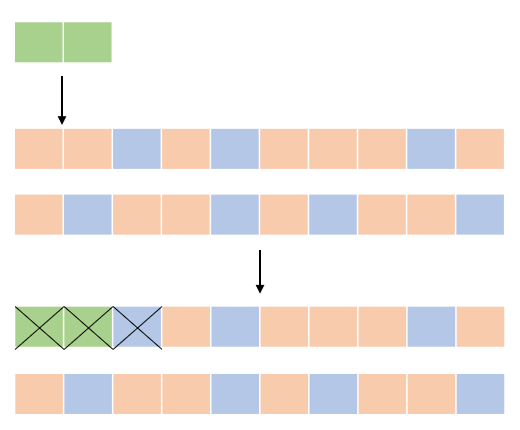
\includegraphics[width=5cm]{./Figures/seat_assign1.png}
%     \caption{Assign The Group in Row 1}
%     \end{minipage}
%     \begin{minipage}[t]{0.48\textwidth}
%     \centering
%     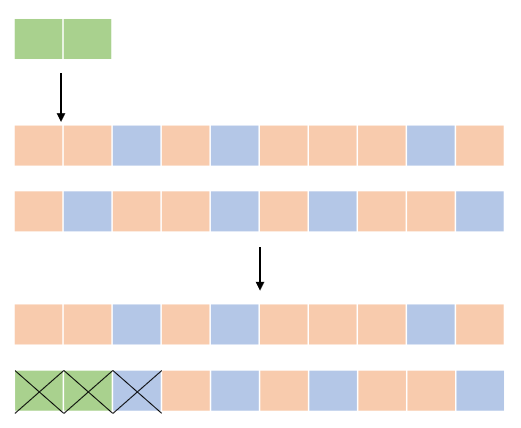
\includegraphics[width=5cm]{./Figures/seat_assign2.png}
%     \caption{Assign The Group in Row 2}
%     \end{minipage}
% \end{figure}


Our main contributions in this paper are summarized as follows. First, this study presents the first attempt to consider the arrangement of seat assignments with social distancing under dynamic arrivals. While many studies in the literature highlight the importance of social distancing in controlling the spread of the virus, they often focus too much on the model and do not provide much insight into the operational significance behind social distancing \cite{barry2021optimal, fischetti2021safe}. Recent studies have explored the effects of social distancing on health and economics, mainly in the context of aircraft \cite{salari2020social, ghorbani2020model, salari2022social}. Our study provides a new perspective to help the government adopt a mechanism for setting seat assignments to implement social distancing during pandemic.

Second, we establish a deterministic model to analyze the effects of social distancing when the demand is known. Due to the medium size of the problem, we can solve the IP model directly. We then develop the scenario-based stochastic programming by considering the stochastic demands of different group types. By using Benders decomposition methods, we can obtain the seat planning quickly. 

Third, to address the problem in the dynamic situation, we first obtain a feasible seat planning from scenario-based stochastic programming. We then make a decision for each incoming group based on our dynamic seat assignment policy, either accepting or rejecting the group. Our results demonstrate a significant improvement over the traditional control policies and provide the insights on the implementation of social distancing.

% Our results demonstrate the effectiveness of our approach in balancing social distancing requirements with revenue generation, providing valuable insights for policymakers and venue managers. Specifically, our proposed approach can help cinemas, concert venues, and other public spaces optimize seat assignments while ensuring the safety of patrons. It provides a practical tool for venues to implement social distancing measures in a flexible and efficient manner, adapting to changes in demand and maximizing revenue generation while maintaining social distancing measures.

% With this new .., we illustrate how to assign the seats by the govenment/stakeholder to balance health and economic issues. In addition, we also provide managerial guidance for the government on how to publish the related policy to make the tradeoff between economic maintenance and risk management.

The rest of this paper is structured as follows. The following section reviews relevant literature. We describe the motivating problem in Section 3. In Section 4, we establish the stochastic model,analyze its properties and obtain the seat planning. Section 5 demonstrates the dynamic seat assignment policy to assign the seats for incoming groups. Section 6 gives the numerical results and the insights of implementing social distancing. The conclusions are shown in Section 7.
\newpage


% % !TEX root = sum1.tex
\section{Literature Review}

The present study is closely connected to the following research areas -- seat planning with social distancing and dynamic seat assignment. The subsequent sections review literature pertaining to each perspective and highlight significant differences between the present study and previous research.


\subsection{Seat Planning with Social Distancing}
Since the outbreak of covid-19, social distancing is a well-recognized and practiced method for containing the spread of infectious diseases \cite{moosa2020effectiveness}. An example of operational guidance is ensuring social distancing in seat plannings.
% particularly in social distancing measures that involve operational details. 

Social distancing in seat planning has attacted considerable attention from the research area. The applications include the allocation of seats on airplanes \cite{ghorbani2020model}, classroom layout planning \cite{bortolete2022support}, seat planning in long-distancing trains \cite{haque2022optimization}. The social distancing can be implemented in various forms, such as fixed distances or seat lengths. Fischetti et al.\cite{fischetti2021safe} consider how to plant positions with social distancing in restaurants and beach umbrellas. Different venues may require different forms of social distancing; for instance, on an airplane, the distancing between seats and the aisle must be considered \cite{salari2022social}, while in a classroom, maximizing social distancing between students is a priority \cite{bortolete2022support}.

These researchs focus on the static version of the problem. This typically involves creating an IP model with social distancing constraints \cite{bortolete2022support, ghorbani2020model, haque2022optimization}, which is then solved either heuristically or directly. The seat allocation of the static form is useful for fixed people, for example, the students in one class. But it is not be practical for the dynamic arrivals in commercial events.


% and family-group seat selection in a theater. \cite{fischetti2021safe}


% Dynamic seat assignment with social distancing can be implemented manually by the venue staff, or through automated systems that use algorithms to optimize the seating arrangements based on various factors, such as the number of available seats, customer preferences, and the recommended distancing between audience members.

% \subsection{Group seat reservation}
The recent pandemic has shed light on the benefits of group reservations, as they have been shown to increase revenue without increasing the risk of infection \cite{moore2021seat}. In our specific setting, we require that groups be accepted on an all-or-none basis, meaning that members of the same family or group must be seated together. However, the group seat reservation policy poses a significant challenge when it comes to determining the seat assignment policy.


This group seat reservation policy has various applications in industries such as hotels \cite{li2013modeling}, working spaces\cite{fischetti2021safe}, public transport\cite{deplano2019offline}, sports arenas\cite{kwag2022optimal}, and large-scale events \cite{lewis2016creating}. This policy has significant impacts on passenger satisfaction and revenue, with the study \cite{yuen2002group} showing that passenger groups increase revenue by filling seats that would otherwise be empty. Traditional works \cite{clausen2010off, deplano2019offline}in transportation focus on maximizing capacity utilization or reducing total capacity needed for passenger rail, typically modeling these problems as knapsack or binpacking problems.

Some related literature mentioned the seat planning under pandemic for groups are represented below.
Fischetti et al. \cite{fischetti2021safe} proposed a seating planning for known groups of customers in amphitheaters. Haque and Hamid \cite{haque2022optimization} considers grouping passengers with the same origin-destination pair of travel and assigning seats in long-distance passenger trains. Salari et al. \cite{salari2022social} performed group seat assignment in airplanes during the pandemic and found that increasing passenger groups can yield greater social distancing than single passengers. Haque and Hamid \cite{haque2023social} aim to optimize seating assignments on trains by minimizing the risk of virus spread while maximizing revenue. The specific number of groups in their models is known in advance. But in our study, we only know the arrival probabilities of different groups.

This paper \cite{blom2022filling} discusses strategies for filling a theater by considering the social distancing and group arrivals, which is similar to ours. However, unlike our project, it only focuses on a specific location layout and it is still based on a static situation by giving the proportion of different groups.

% In contrast, there is a lack of research on group seat reservations for booking tickets for cinemas, where available seats are typically displayed for customers to choose from for low-demand movie tickets. For concerts with high demand, it is usually not possible to choose seats independently, and the organizer will inform seat information after confirming the order. 
% For movies of the same time period, the ticket prices are the same, while for the same concert, although there are different ticket prices, for the same region, the ticket prices are the same. Therefore, we can consider different ticket prices separately. 
% In the absence of an epidemic, all requests for tickets can be considered one by one. However, the COVID-19 pandemic has shed new light on the potential benefits of group reservations, as they can improve revenue without increasing the risk of infection. 


% Dundar and Karakose \cite{dundar2021seat} proposed a two-stage algorithm for classroom seat assignment during the pandemic, with the first phase maximizing total allocations and the second phase maximizing the minimum interpersonal distance between students. 


\subsection{Dynamic Seat Assignment}
Our model in its static form can be viewed as a specific instance of the multiple knapsack problem \cite{pisinger1999exact}, where we aim to assign a subset of groups to some distinct rows. 


In our dynamic form, the decision to accept or reject groups is made at each stage as they arrive. The related problem can be dynamic knapsack problem \cite{kleywegt1998dynamic}, where there is one knapsack.

% and dynamic bin-packing problem \cite{coffman1983dynamic, berndt2020fully} where items arrive and depart online and all knapsacks are the same. 

% However, solving this problem is strongly NP-hard, which means that finding an optimal solution for large instances of the problem is computationally challenging \cite{pisinger1999exact}.

Dynamic seat assignment is a process of assigning seats to passengers on a transportation vehicle, such as an airplane, train, or bus, in a way that maximizes the efficiency and convenience of the seating arrangements \cite{hamdouch2011schedule, berge1993demand, zhu2023assign}. 

Our problem is closely related to the network revenue management (RM) problem \cite{williamson1992airline}, which is typically formulated as a dynamic programming (DP) problem. However, for large-scale problems, the exponential growth of the state space and decision set makes the DP approach computationally intractable. To address this challenge, we propose using scenario-based programming \cite{feng2013scenario, casey2005scenario, henrion2018problem} to determine the seat planning. In this approach, the aggregated supply can be considered as a protection level for each group type. Notably, in our model, the supply of larger groups can also be utilized by smaller groups. This is because our approach focuses on group arrival rather than individual unit, which sets it apart from traditional partitioned and nested approaches \cite{curry1990optimal, van2008simulation}.


We have two distinct features: group-based and assignment.

Traditional revenue management focuses on decision-making issues, namely accepting or rejecting a request \cite{gallego1997multiproduct}.However, our paper not only addresses decision-making, but also emphasizes the significance of assignment, particularly in the context of seat assignment. This sets it apart from traditional revenue management methods and makes the problem more challenging.

Similarly, the assign-to-seat feature introduced by Zhu et al. \cite{zhu2023assign} also highlights the importance of seat assignment in revenue management. This trait addresses the challenge of selling high-speed train tickets in China, where each request must be assigned to a single seat for the entire journey and takes into account seat reuse. This further emphasizes the significance of seat assignment and sets it apart from traditional revenue management methods.


% The authors propose a modified network revenue management model and introduce a bid-price control policy based on a novel maximal sequence principle. They also propose a "re-solving a dynamic primal" policy that achieves uniformly bounded revenue loss. The study reveals connections between this problem and traditional network revenue management problems and shows that the impact of the assign-to-seat restriction can be limited with the proposed methods.


% Jiang et al. \cite{jiang2015dynamic} proposes a revenue management approach for high-speed rail (HSR) passenger ticket assignment with dynamic adjustments. The approach integrates short-term demand forecasting, ticket assignment, and dynamic ticket adjustment mechanisms to allocate passenger tickets during presale periods and avoid situations where tickets are insufficient at some stations while seats remain empty.



% Implementing dynamic seat assignment with social distancing can be done manually by the staff or through automated systems that use algorithms to optimize the seat assignments based on various factors, such as ticket sales, seat availability, and customer preferences. However, the implementation of social distancing measures poses unique challenges that require careful planning and consideration of various factors to balance safety with revenue generation.


% \subsection{Scenario generation}

% It is challenging to consider all the possible realizations; thus, it is practicable to use discrete distributions with a finite number of scenarios to approximate the random demands. This procedure is often called scenario generation.

% Some papers consider obtaining a set of scenarios that realistically represents the distributions of the random parameters but is not too large. \cite{feng2013scenario} \cite{casey2005scenario}
% \cite{henrion2018problem}

% Another process to reduce the calculation is called scenario reduction. It tries to approximate the original scenario set with a smaller subset that retains essential features.



% Every time we can regenerate the scenario based on the realized demands. (Use the conditional distribution or the truncated distribution)


% Suppose that the groups arrive from small to large according to their size. Once a larger group comes, the smaller one will never appear again.

% When a new group arrives (suppose we have accepted $n$ groups with the same size), we accept or reject it according to the supply (when $n+1 < \text{supply}$, we accept it). 
% then update the scenario set according to the truncated distribution. We can obtain a new supply with the new probability and scenario set.


\newpage


% !TeX root = ../main.tex

\section{Seat Planning with Deterministic Demand}
    \frame{\sectionpage}

  \begin{frame}{Deterministic Formulation}  %开始一张幻灯片
    Seat planning problem with given demand $\bm{d}$:

    \begin{equation}\label{deter_upper}
      \begin{aligned}
      \max \quad & \sum_{i=1}^{M}  \sum_{j= 1}^{N} (n_i- \delta) x_{ij} \\
      \text {s.t.} \quad & \sum_{j= 1}^{N} x_{ij} \leq d_{i}, \quad i \in \mathcal{M}, \\
      & \sum_{i=1}^{M} n_{i} x_{ij} \leq L_j, j \in \mathcal{N}, \\
      & x_{ij} \in \mathbb{Z}_{+}, \quad i \in \mathcal{M}, j \in \mathcal{N}.
      \end{aligned}
    \end{equation}
    Objective: maximize the number of people accommodated.

    $x_{ij}$: the number of group type $i$ in row $j$.
  \end{frame}

  \begin{frame}{Property}
    In the LP relaxation of problem \eqref{deter_upper}, there exists an index $v$ such that the optimal solutions satisfy the following conditions:

    \begin{itemize}
      \item For $i = 1,\ldots, v-1$ and for all $j$, $x_{ij}^{*} = 0$. 
      % indicating that no group type $i$ are assigned to any rows before index $v$.
      \item For $i = v+1,\ldots, M$, $\sum_{j} x_{ij}^{*} = d_{i}$. 

      \item For $i = v$, $\sum_{j} x_{ij}^{*} = \frac{L - \sum_{i = v+1}^{M} {d_i n_i}}{n_v}$ 
      % This quantity is determined by the available supply, which is calculated as the remaining seats after accommodating the demands for group types $v+1$ to $M$, divided by the size of group type $v$, denoted as $n_v$.
    \end{itemize}

    When the demand is way smaller than the number of seats, the seat planning obtained from problem \eqref{deter_upper} does not utilize all seats. We aim to generate a seat planning utilizing all seats while ensuring that the demand requirements are met.
  \end{frame}

  \begin{frame}{Generate The Full or Largest Pattern}
    Specifically, we can convert a given specific pattern into a largest or full pattern while ensuring that the original group type requirements are met. Our objective is to generate the pattern with maximal people.

    Mathematically, for any pattern $\bm{h} = (h_1, \ldots, h_M)$, we seek to find a pattern $\bm{h}{'} = (h_1{'}, \ldots, h_M{'})$ that satisfies the following programming.

    \begin{equation*}\label{full_largest}
      \begin{aligned}
      \max \quad & |\bm{h}{'}| \\
      \text {s.t.} \quad & h_1{'} \geq h_1 \\
      &  h_1{'} + h_2{'} \geq h_1 + h_2 \\
      & \cdots \\
      & h_1{'} + \ldots + h_M{'} \geq h_1 + \ldots + h_M.
      \end{aligned}
    \end{equation*}
  \end{frame}

  \begin{frame}{Algorithm to Generate The Full or Largest Pattern}
    For each row $j$, let $\beta_{j} = L_{j} - \sum_{i} n_{i} x_{ij}$. We aim to allocate the remaining unoccupied seats($\beta_{j}$) in row $j$ in a way that maximizes the number of planned groups that become the largest in size.
    \vspace{0.5cm}
    
    Allocation scheme of $\beta_{j}$:
    \vspace{0.5cm}

    \begin{scriptsize}
      Let $k = \min\{i | h_i > 0\}$ for a pattern $\bm{h}$.

      \begin{itemize}
        \item If $k \neq M$, $h_{k} \gets h_{k} -1$, $h_{\min_{\{(k+\beta_{j}), M\}}} \gets h_{\min_{\{(k+\beta_{j}), M\}}} +1$, $\beta_{j} \gets \beta_{j} - \max\{1, M - k\}$. Continue this procedure until the pattern is largest or $\beta_{j} =0$.
        \item If $k = M$ and $\beta_{j} > 0$, continue the following procedure until $\beta < n_{1}$.
        \item[-] When $\beta \geq n_{M}$, $q \gets \lfloor\frac{\beta}{n_M}\rfloor$, $\beta_{j} \gets \beta_{j} - q n_M$, $h_{M} \gets h_{M} + q$.
        \item[-] When $n_{1} \leq \beta_{j} < n_{M}$, $h_{\beta_{j}-n_1+1} \gets h_{\beta_{j}-n_1+1} + 1$, $\beta_{j} \gets 0$.
        % \item[] assign $\beta$ in a greedy way.
      \end{itemize}  
    \end{scriptsize}
    
  \end{frame}

% !TeX root = ../main.tex

\section{Stochastic Demand Situation}
    \frame{\sectionpage}

    \begin{frame}{Method Flow}
      We aim to obtain a seat planning before the demand realization.
      \begin{itemize}
        \item The formulation of scenario-based stochastic programming(SSP).
        \item Reformulate SSP to the benders master problem(BMP) and subproblem.
        \item The optimal solution can be obtained by solving BMP iteratively.
        \item To avoid solving IP directly, we consider the linear relaxation form.
        \item Obtain integral seat planning composed of full or largest patterns by deterministic model.
      \end{itemize}
    \end{frame}

    \begin{frame}{Scenario-based Stochastic Programming}
      \footnotesize
      \begin{equation}\label{sto_form}
        \begin{aligned}
       (SSP) \max \quad & E_{\omega}\left[\sum_{i=1}^{M-1} (n_i-\delta) (\sum_{j= 1}^{N} x_{ij} + y_{i+1,\omega}^{+} - y_{i \omega}^{+}) + (n_{M}-\delta) (\sum_{j= 1}^{N} x_{Mj} - y_{M \omega}^{+})\right] \\
        \text {s.t.} \quad & \sum_{j= 1}^{N} x_{ij}-y_{i \omega}^{+}+
        y_{i+1, \omega}^{+} + y_{i \omega}^{-}=d_{i \omega}, \quad i = 1,\ldots,M-1, \omega \in \Omega \\
        & \sum_{j= 1}^{N} x_{ij} -y_{i \omega}^{+}+y_{i \omega}^{-}=d_{i \omega}, \quad i = M, \omega \in \Omega \\
        & \sum_{i=1}^{M} n_{i} x_{ij} \leq L_j, j \in \mathcal{N}\\
        & y_{i \omega}^{+}, y_{i \omega}^{-} \in \mathbb{Z}_{+}, \quad i \in \mathcal{M}, \omega \in \Omega \\
        & x_{ij} \in \mathbb{Z}_{+}, \quad i \in \mathcal{M}, j \in \mathcal{N}.
        \end{aligned}
      \end{equation}
    \end{frame}

\begin{frame}{Reformulation}
  \begin{equation}\label{BD_master}
    \begin{aligned}
  \max \quad & \mathbf{c}^{\intercal} \mathbf{x}+ z(\mathbf{x}) \\
  \text {s.t.} \quad & \mathbf{n} \mathbf{x} \leq \mathbf{L} \\
  & \mathbf{x} \in \mathbb{Z}_{+}^{M \times N},
  \end{aligned}
  \end{equation}

  where $z(\mathbf{x})$ is defined as 

$$z(\mathbf{x}) := E(z_{\omega}(\mathbf{x})) = \sum_{\omega \in \Omega} p_{\omega} z_{\omega}(\mathbf{x}),$$ and for each scenario $\omega \in \Omega$, 

  \begin{equation}\label{BD_sub}
    \begin{aligned}
      z_{\omega}(\mathbf{x}) := \max \quad & \mathbf{f}^{\intercal} \mathbf{y} \\
      \text {s.t.} \quad & \mathbf{x} \mathbf{1} + \mathbf{V} \mathbf{y} = \mathbf{d}_{\omega} \\
       & \mathbf{y} \geq 0.
    \end{aligned}
    \end{equation}
\end{frame}

\begin{frame}{Solution to Subproblem}
  Problem (3) is easy to solve with a given $\mathbf{x}$ which can be seen by the dual problem:

  \begin{equation}\label{BD_sub_dual}
    \begin{aligned}
      \min \quad & \alpha^{\intercal}_{\omega} (\mathbf{d}_{\omega}- \mathbf{x} \mathbf{1}) \\
      \text {s.t.} \quad & \alpha^{\intercal}_{\omega} \mathbf{V} \geq \mathbf{f}^{\intercal}
    \end{aligned}
    \end{equation}

    \begin{itemize}
      \item The feasible region of problem \eqref{BD_sub_dual}, $P= \{\alpha|\alpha^{\intercal} V \geq \mathbf{f}^{\intercal}\}$, is bounded. In addition, all the extreme points of $P$ are integral.
      \item The optimal solution to this problem can be obtained directly according to the complementary slackness property.
    \end{itemize}
\end{frame}

\begin{frame}{Benders Decomposition Procedure}
  \small
  Let $z_{\omega}$ be the lower bound of problem \eqref{BD_sub_dual}, SSP can be obtained by solving following restricted benders master problem:
  \begin{equation}\label{BD_master2}
    \begin{aligned}
      \max \quad & \mathbf{c}^{\intercal} \mathbf{x} + \sum_{\omega \in \Omega} p_{\omega} z_{\omega} \\
      \text {s.t.} \quad & \mathbf{n} \mathbf{x} \leq \mathbf{L} \\
      & (\alpha^{k})^{\intercal}(\mathbf{d}_{\omega}- \mathbf{x} \mathbf{1}) \geq z_{\omega}, \alpha^k \in \mathcal{O}, \forall \omega \\
       & \mathbf{x} \in \mathbb{Z}_{+}
    \end{aligned}
\end{equation} 

  Constraints will be generated from problem \eqref{BD_sub_dual} until an optimal solution is found.

  \begin{figure}[ht]
    \centering
    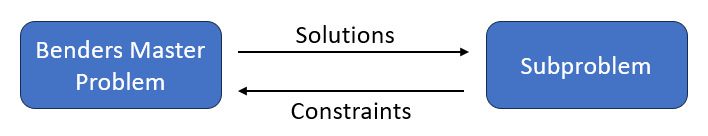
\includegraphics[width = 0.6\textwidth]{./images/BD.png}
  \end{figure}

  To avoid solving IP directly, we consider the linear relaxation of Problem \eqref{BD_master2}.
\end{frame}

% \begin{frame}{Deterministic Formulation}
%   Substitute the first constraint with $\sum_{j= 1}^{N} x_{ij} \geq s_{i}, i \in \mathcal{M}$, we can obtain the problem with lower bound supply. 
% \end{frame}

\begin{frame}{Obtain Seat Planning Composed of Full or Largest Patterns}
      \begin{description}
        \item[Step 1.] Obtain the solution, $\mathbf{x}^{*}$, by benders decomposition. Aggregate $\mathbf{x}^{*}$ to the number of each group type, ${s}_{i}^{0} =\sum_{j} x^{*}_{ij}, i \in \mathbf{M}$.

        \item[Step 2.] Solve problem \eqref{deter_upper} to obtain the optimal solution, $\mathbf{x}^{1}$. Aggregate $\mathbf{x}^{1}$ to the number of each group type, ${s}_{i}^{1} = \sum_{j} x^{1}_{ij}, i \in \mathbf{M}$.
         
        \item[Step 3.] For each row, construct a full or largest pattern.
     \end{description}
\end{frame}

\begin{frame}{Construction}
There exists an optimal solution to the stochastic programming problem such that the patterns associated with this optimal solution are composed of the full or largest patterns under any given scenarios.

Algorithm to obtain the solution of problem \eqref{full_largest}.
\end{frame}

\begin{frame}{Verify the performance}
  To verify the performance of the seat planning obtained from stochastic programming, we 

  % under the setting of fixed seat planning
\end{frame}

\section{Seat Assignment with Dynamic Requests}\label{sec_dynamic_seat}

In many commercial situations, requests arrive sequentially over time, and the seller must immediately decide whether to accept or reject each request upon arrival while ensuring compliance with the required spacing constraints. If a request is accepted, the seller must also determine the specific seats to assign. Importantly, each request must be either fully accepted or entirely rejected; once seats are assigned to a group, they cannot be altered or reassigned to other requests.

To model this problem, we formulate it using dynamic programming approach in a discrete-time framework. Time is divided into $T$ periods, indexed forward from $1$ to $T$. We assume that in each period, at most one request arrives and the probability of an arrival for a group type $i$ is denoted as $p_i$, where $i \in \mathcal{M}$. The probabilities satisfy the constraint $\sum_{i=1}^M p_i \leq 1$, indicating that the total probability of any group arriving in a single period does not exceed one. We introduce the probability $p_0 = 1 - \sum_{i=1}^{M} p_i$ to represent the probability of no arrival in each period. To simplify the analysis, we assume that the arrivals of different group types are independent and the arrival probabilities remain constant over time. This assumption can be extended to consider dependent arrival probabilities over time if necessary.

The remaining capacity in each row is represented by a vector $\mathbf{L} = (l_1, l_2, \ldots, l_N)$, where $l_j$ denotes the number of remaining seats in row $j$. Upon the arrival of a group type $i$ at time $t$, the seller needs to make a decision denoted by $u_{i,j}^{t}$, where $u_{i,j}^{t} = 1$ indicates acceptance of group type $i$ in row $j$ during period $t$, while $u_{i,j}^{t} = 0$ signifies rejection of that group type in row $j$. The feasible decision set is defined as $$U^{t}(\mathbf{L}) = \left\{u_{i,j}^{t} \in \{0,1\}, \forall i \in \mathcal{M}, \forall j \in \mathcal{N} \bigg| \sum_{j=1}^{N} u_{i,j}^{t} \leq 1, \forall i \in \mathcal{M}; n_{i}u_{i,j}^{t}\mathbf{e}_j \leq \mathbf{L}, \forall i \in \mathcal{M}, \forall j \in \mathcal{N}\right\}.$$
Here, $\mathbf{e}_j$ represents an N-dimensional unit column vector with the $j$-th element being 1, i.e., $\mathbf{e}_j = (\underbrace{0, \cdots, 0}_{j-1}, 1, \underbrace{0, \cdots, 0}_{N-j})$. The decision set $U^{t}(\mathbf{L})$ consists of all possible combinations of acceptance and rejection decisions for each group type in each row, subject to the constraints that at most one group of each type can be accepted in any row, and the number of seats occupied by each accepted group must not exceed the remaining capacity of the row.

Let $V^{t}(\mathbf{L})$ denote the maximum expected revenue earned by the optimal decision regarding group seat assignments at the beginning of period $t$, given the remaining capacity $\mathbf{L}$. Then, the dynamic programming formulation for this problem can be expressed as:

\begin{equation}\label{DP}
V^{t}(\mathbf{L}) = \max_{u_{i,j}^{t} \in U^{t}(\mathbf{L})}\left\{\sum_{i=1}^{M} p_i \bigl( \sum_{j=1}^{N} i u_{i,j}^{t} + V^{t+1}(\mathbf{L} - \sum_{j=1}^{N} n_i u_{i,j}^{t}\mathbf{e}_j)\bigr) + p_0 V^{t+1}(\mathbf{L})\right\}
\end{equation}
with the boundary conditions $V^{T+1}(\mathbf{L}) = 0, \forall \mathbf{L}$, which implies that the revenue at the last period is 0 under any capacity. The initial capacity is denoted as $\mathbf{L}_{0} = (L_1, L_2, \ldots, L_N)$. Our objective is to determine group assignments that maximize the total expected revenue during the horizon from period 1 to $T$, represented by $V^{1}(\mathbf{L}_{0})$.


Solving the dynamic programming problem in equation \eqref{DP} presents computational challenges due to the curse of dimensionality that arises from the large state space. To address this, we develop a relaxed dynamic programming formulation and propose the Seat-Plan-Based Assignment (SPBA) policy. This policy combines the relaxed DP for preliminary acceptance decisions with the seat plan that serves as the basis for the final assignment decision.

% We propose our policy for assigning arriving requests in a dynamic context. First, we employ relaxed dynamic programming to determine whether to prepare a request for assignment or to reject it. Then, we develop the seat assignment approach based on the seat plan generated from Section \ref{sec_seat_planning}.


\subsection{Seat-Plan-Based Assignment}
The Seat-Plan-Based Assignment (SPBA) policy dynamically allocates groups through a two-stage process. In the first stage, requests are evaluated using relaxed dynamic programming (RDP). The second stage, known as group-type control, initially accepted requests are verified and assigned based on expected future revenue, considering the current seat plan and remaining time periods. As part of this stage, accepted requests are further assigned to specific rows according to tie-breaking rules. To enhance computational efficiency and avoid regenerating the seat plan in every period, we establish specific criteria for determining when to update the seat plan.

% In addition, we present alternative policies to facilitate comparative performance analysis.

\subsubsection{Relaxed Dynamic Programming}
To simplify the complexity of the dynamic programming formulation in \eqref{DP}, we employ a relaxed dynamic programming (RDP) approach by aggregating all rows into a single row with the total capacity $\tilde{L} = \sum_{j=1}^{N} L_j$. This relaxation yields preliminary seat assignment decisions for each group arrival, where the rejection by the RDP is final (no further evaluation is needed), the acceptance by the RDP is tentative and must be validated according to the current seat plan in the subsequent group-type control.

Let $u_{i}^{t} \in $ denote the RDP's decision variable for accepting ($u_{i}^{t} = 1$) or rejecting ($u_{i}^{t} = 0$) a type $i$ request in period $t$. The value function of the relaxed DP with the total capacity $l$ in period $t$, denoted by $V^{t}(l)$, is the following:

\begin{equation}\label{DP_relaxed}
V^{t}(l) =  \max_{u_{i}^{t} \in \{0,1\}} \left\{ \sum_{i=1}^{M} p_i \left[V^{t+1}(l-n_i u_{i}^{t})+ i u_{i}^{t}\right] + p_0 V^{t+1}(l)\right\}
\end{equation}
with the boundary conditions $V^{T+1}(l) =0, \forall l \geq 0$ and $V^{t}(0) =0, \forall t$.


To make the initial decision, we compute the value function $V^{t}(l)$ and compare the values of accepting versus rejecting the request. Preliminarily accepted requests are then verified and assigned in the subsequent group-type control stage.

% However, the RDP policy alone cannot guide an effective assignment approach. We proceed with the assignment by the following group-type control.


% {\color{red}{The last sentence is not clear. You should explain how this relaxed DP will be used later in the seat assignment.}}

% Two-stage: initial acceptance, then assignment?

% Note that we must first verify whether the group can be accommodated with the available seats. Specifically, if the size of the arriving group exceeds the maximum remaining capacity across all rows, the group must be rejected. Once a group is accepted, the next step is to determine where to assign the seats. However, in the absence of a specific seat plan, there are no predefined rules to guide this assignment process. To address this, we adopt a rule similar to the Best Fit rule \citep{johnson1974fast}. Specifically, the group is assigned to the row with the smallest remaining seats that can still accommodate the group.

% To determine whether to assign the arriving group and which row to place it in when the DP approach accepts the group, we developed a group-type control policy.

\subsubsection{Group-Type Control}\label{nested_policy}
The group-type control allocation verifies and assigns requests initially accepted in the first stage. It assesses whether the current seat plan can accommodate the arriving group while balancing the trade-off between preserving seat availability for potential future requests and accepting the current request. To make this decision, we compare the expected number of acceptable individuals for both options. Accepted requests are then assigned to specific rows based on tie-breaking rules.

% When a group is accepted and assigned to larger-size seats, the remaining empty seat(s) can be reserved for future demand without affecting the rest of the seat plan. To determine whether to use larger seats to accommodate the incoming group, we compare the expected number of acceptable individuals of accepting the group in the larger seats and rejecting the group based on the current seat plan. Then we identify the possible rows where the incoming group can be assigned based on the group types and seat availability.

Specifically, suppose the supply at period $t$ is $[X_1^{t}, \ldots, X_M^{t}]$, with $(T-t)$ remaining periods. A request of type $i$ arrives and is initially accepted in the first stage. If $X_{i}^{t} > 0$, the request is accepted directly. If $X_{i}^{t} = 0$, the request can still be accepted by utilizing one unit of supply from group type $\hat{i}$ for any $\hat{i}={i}+1, \ldots, M$. 
\begin{itemize}
  \item When $\hat{i} = {i}+\delta+1, \ldots, M$, the remaining $(\hat{i}-{i}-\delta)$ seats can be allocated to one additional group type $(\hat{i}-{i}-\delta)$, ensuring the social distancing of $\delta$ seats.
  \item When $\hat{i} = {i}+1, \ldots, i+\delta$, the expected number of accepted individuals is ${i}$, while the remaining $\hat{i}-{i}$ seats beyond the accepted group are wasted.
\end{itemize}

Let $D_{\hat{i}}^{t}$ be the random variable representing the number of future arrivals of group type $\hat{i}$ in the remaining $t$ periods. The expected number of accepted individuals is given by: $${i} + (\hat{i}-{i}-\delta)P(D_{\hat{i}-{i}-\delta}^{T-t} \geq X_{\hat{i}-{i}-\delta}^{t}+1),$$ where $P(D_{i}^{T-t} \geq X_{i}^{t})$ represents the probability that  demand for group type ${i}$ in the remaining $(T-t)$ periods meets or exceeds the current remaining supply $X_{i}^{t}$. Thus, the term, $P(D_{\hat{i}-{i}-\delta}^{T-t} \geq X_{\hat{i}-{i}-\delta}^{t}+1)$, specifically captures the probability that demand for group type $(\hat{i}-{i}-\delta)$ in future periods exceeds its current remaining supply by at least one unit.

Similarly, if we reject the current group type $i$ to preserve capacity for potential future groups of type $\hat{i}$, the expected number of accepted individuals becomes: $$\hat{i} P(D_{\hat{i}}^{T-t} \geq X_{\hat{i}}^{t}),$$ where $P(D_{\hat{i}}^{T-t} \geq X_{\hat{i}}^{t})$ represents the probability that the demand for group type $\hat{i}$ during the remaining $(T-t)$ periods meets or exceeds its current remaining supply $X_{\hat{i}}^{t}$.

Let $d^{t}({i},\hat{i})$ denote the difference of the expected number of accepted individuals between accepting a group type ${i}$ (occupying $(\hat{i}+\delta)$-size seats) and rejecting it in period $t$. This difference is given by:
\begin{equation*}
	d^{t}({i},\hat{i}) = \begin{cases}
    {i} + (\hat{i}-{i}-\delta)P(D_{\hat{i}-{i}-\delta}^{T-t} \geq X_{\hat{i}^{t}-{i}-\delta}^{t}+1) - \hat{i} P(D_{\hat{i}}^{T-t} \geq X_{\hat{i}}^{t}), &\text{if}~ \hat{i} = {i}+\delta+1, \ldots, M, \\
    {i} - \hat{i} P(D_{\hat{i}}^{T-t} \geq X_{\hat{i}}^{t}), &\text{if}~ \hat{i} = {i}+1, \ldots, {i}+\delta.
		\end{cases}
\end{equation*}

The optimal decision selects $\hat{i}^{*} = \arg \max_{\hat{i} = {i}+1, \ldots, M} d^{t}({i},\hat{i})$. The group is accepted and assigned to $(\hat{i}^{*} + \delta)$-size seats if $d^{t}({i},\hat{i}^{*}) \geq 0$, otherwise rejected. After determining the optimal group type $\hat{i}^{*}$, we apply the tie-breaking rule to assign the request to a specific row that includes group type $\hat{i}^{*}$.

% {\color{red}{how is this related to group type control?}}

\subsubsection*{Tie-Breaking for Row Selection}\label{tie-break}
A tie occurs when there are several rows to assign the request. To determine the appropriate row for seat assignment, we can apply the following tie-breaking rules among the possible options. Suppose one request of type ${i}$ arrives, the current seat plan is $\bm{H} = [\bm{h}_{1}^{\intercal}, \ldots, \bm{h}_{N}^{\intercal}]$, the corresponding supply is $\bm{X}$. Let $s_{j} = L_j - \sum_{i =1}^{M} n_{i} H_{ij}$ represent the remaining number of seats in row $j$ after considering the seat allocation for the assigned requests. When $X_{i} > 0$, we assign the request to row $k \in \arg \min_{j \in \mathcal{N}} \{s_{j}|H_{ij} > 0\}$ such that the row can be filled as much as possible. When $X_{i} = 0$ and the request is accepted to take the seats planned for type $\hat{i}, \hat{i}>i$, we assign the request to a row $k \in \arg \max_{j \in \mathcal{N}} \{s_{j}| H_{\hat{i} j}>0\}$. That can help reduce the number of rows that are not full. When there are multiple $k$s available, we can choose one arbitrarily. 

% This rule in both scenarios prioritizes filling rows and leads to better seat management.

% As an example to illustrate group-type control and the tie-breaking rule, consider a situation where $L_1 =3, L_2 = 4, L_3 =5, L_4 =6$, $M =4$, $\delta =1$. The corresponding patterns for each row are $(0,1,0,0)$, $(0,0,1,0)$, $(0,0,0,1)$ and $(0,0,0,1)$, respectively. Thus, $\beta_1 = \beta_2 = \beta_3 =0$, $\beta_4 =1$. Now, a group type 1 arrives, and the group-type control indicates the possible rows where the group can be assigned. We assume this group can be assigned to the seats of the largest group according to the group-type control, then we have two options: row 3 or row 4. To determine which row to select, we can apply the tie-breaking rule. The $\beta$ value of the rows will be used as the criterion, we would choose row 4 because $\beta_4$ is larger. Because when we assign it in row 4, there will be two seats reserved for future group type 1, but when we assign it in row 3, there will be one seat remaining unused.

% In the above example, the group type 1 can be assigned to any row with the available seats. The group-type control can help us find the larger group type that can be used to place the arriving group while maximizing the expected values. When there are multiple rows containing the larger group type, we choose the row containing the larger group type according to the tie-breaking rule.

% Combining the group-type control strategy with the evaluation of relaxed DP values, we obtain a comprehensive decision-making process within a single period. This integrated approach enables us to make informed decisions regarding the acceptance or rejection of incoming requests, as well as determine the appropriate row for the assignment when acceptance is made. 

\subsubsection{Regenerating the Seat Plan}
A useful technique often applied in network revenue management to enhance performance is re-solving \citep{secomandi2008analysis, jasin2012re}, which, in our context, corresponds to regenerating the seat plan. However, to optimize computational efficiency, it is unnecessary to regenerate the seat plan for every request. Instead, we adopt a more streamlined approach. Since seats allocated for the largest group type can accommodate all smaller group types, the seat plan must be regenerated when the supply for the largest group type reaches zero. This ensures that the largest group type is not rejected due to infrequent updates. Additionally, regeneration is required after determining whether to assign the arriving group to seats originally planned for larger groups. By regenerating the seat plan in these specific situations, we integrate real-time information into seat assignment while reducing the frequency of planning updates, thereby balancing efficiency and effectiveness.

The algorithm for regenerating the seat plan is outlined below.

\begin{algorithm}[H]
  \caption{Seat-Plan-Based Assignment}
  Obtain $\bm{X}^{1}$ and $\bm{H}^{1}$ from Algorithm \ref{seat_construction}, calculate $V^{t}(l)$ by \eqref{DP_relaxed}, $\forall t =2, \ldots, T; \forall l = 1,2, \ldots, \tilde{L}$\;
  \For{$t =1, \ldots, T$}
  {Observe a request of group type ${i}$\;
    \eIf{$V^{t+1}(l^{t}) \leq V^{t+1}(l^{t}-n_i) + i$}
    {\eIf{$X_{i}^{t} > 0$}
    {Set $k = \arg \min_{j \in \mathcal{N}} \{L_j^{t} - \sum_{i=1}^{M} n_i H^{t}_{ij}|H^{t}_{ij} >0\}$, break ties arbitrarily\; 
     Assign the group in row $k$, let $L_{k}^{t+1} \gets L_{k}^{t}- n_{i}$, $l^{t+1} \gets l^{t}-n_{i}$, $H_{ik}^{t+1} \gets H_{ik}^{t}-1$, $X_{i}^{t+1}\gets X_{i}^{t}-1$\;
    \If{${i} = M$ and $X_{M}^{t} =0$}
    {Generate seat plan $\bm{H}^{t+1}$ from Algorithm \ref{seat_construction}, update the corresponding $\bm{X}^{t+1}$\;}}
    {Calculate $d^{t}({i}, \hat{i}^{*})$\;
    \eIf{$d^{t}({i}, \hat{i}^{*}) \geq 0 $}
    {Set $k = \arg \max_{j \in \mathcal{N}} \{L_j^{t} - \sum_{i=1}^{M} n_i H_{ij}^{t}|H_{\hat{i}^{*} j}^{t} >0\}$, break ties arbitrarily\;
     Assign the group in row $k$, let $L_{k}^{t+1} \gets L_{k}^{t}- n_{i}$, $l^{t+1} \gets l^{t}-n_{i}$\;
    Generate seat plan $\bm{H}^{t+1}$ from Algorithm \ref{seat_construction}, update the corresponding $\bm{X}^{t+1}$\;}
    {Reject the group and let $L_{k}^{t+1} \gets L_{k}^{t}$, $l^{t+1} \gets l^{t}$\;}}}
    {Reject the group and let $L_{k}^{t+1} \gets L_{k}^{t}$, $l^{t+1} \gets l^{t}$\;}}
\end{algorithm}

% {\color{red}{we may move these alternative policies into appendix}}


% !TeX root = ../main.tex

      
    \begin{frame}{Performances of Different Policies}
        \scriptsize
        $M =4$, $\delta =1$, $N =10$, $L_j =21, j \in \mathcal{N}$, $p_0 = 0$, $|\Omega| = 1000$.
        \begin{table}[ht]
          \centering
          \begin{tabular}{|l|l|l|l|l|l|l|}
          \hline
           T & Probabilities & DSA (\%) & DP1 (\%) & Bid (\%) & Booking (\%) & FCFS (\%) \\
          \hline
          60  & [0.25, 0.25, 0.25, 0.25]  & 99.12 & 98.42 & 98.38 & 96.74 & 98.17 \\
          70  &   & 98.34 & 96.87 & 96.24 & 97.18 & 94.75 \\
          80  &   & 98.61 & 95.69 & 96.02 & 98.00 & 93.18 \\
          90  &   & 99.10 & 96.05 & 96.41 & 98.31 & 92.48 \\
          100 &   & 99.58 & 95.09 & 96.88 & 98.70 & 92.54 \\
          \hline
          60  & [0.25, 0.35, 0.05, 0.35]  & 98.94 & 98.26 & 98.25 & 96.74 & 98.62 \\
          70  &   & 98.05 & 96.62 & 96.06 & 96.90 & 93.96 \\
          80  &   & 98.37 & 96.01 & 95.89 & 97.75 & 92.88 \\
          90  &   & 99.01 & 96.77 & 96.62 & 98.42 & 92.46 \\
          100 &   & 99.23 & 97.04 & 97.14 & 98.67 & 92.00 \\
          \hline
          60  & [0.15, 0.25, 0.55, 0.05]  & 99.14 & 98.72 & 98.74 & 96.61 & 98.07 \\
          70  &   & 99.30 & 96.38 & 96.90 & 97.88 & 96.25 \\
          80  &   & 99.59 & 97.75 & 97.87 & 98.55 & 95.81 \\
          90  &   & 99.53 & 98.45 & 98.69 & 98.81 & 95.50 \\
          100 &   & 99.47 & 98.62 & 98.94 & 98.90 & 95.25 \\
          \hline
          \end{tabular}
        \end{table}
        DSA has better performance than other policies under different demands.

    \end{frame}
      
    \begin{frame}{Impact of Social Distancing as Demand Increases}
        \scriptsize
        $\gamma = p_1 * 1 + p_2 * 2 + p_3 * 3 + p_4 * 4$: the expected number of people at each period.
        \begin{figure}[h]
            \centering
            \subfigure[When $\gamma =2.5$]{
              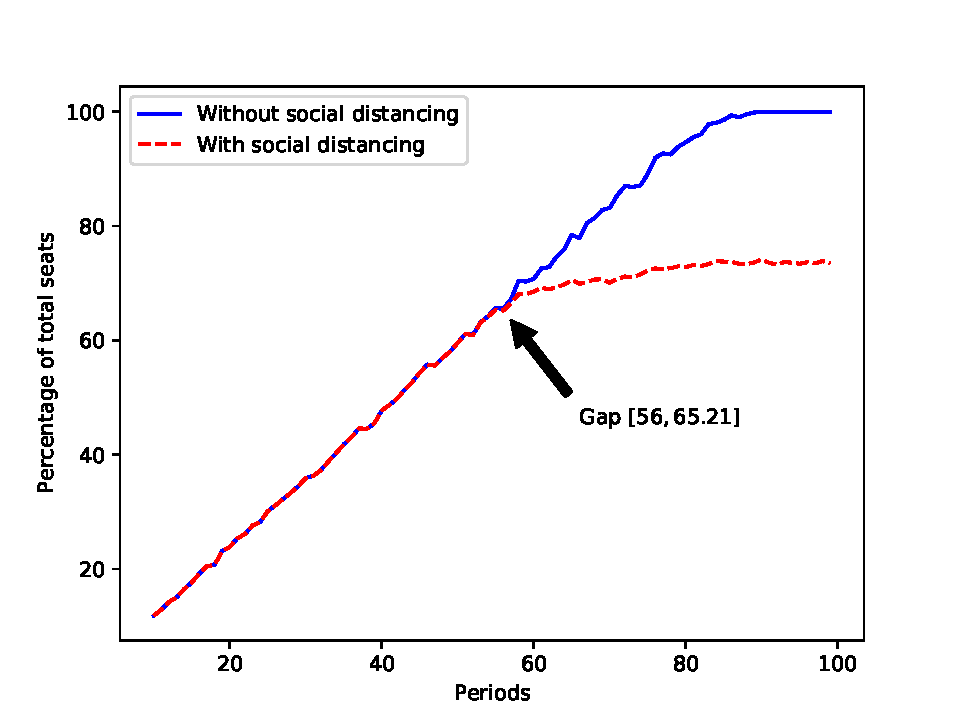
\includegraphics[width=0.48\textwidth]{./images/p1.pdf}}
            \subfigure[When $\gamma =1.9$]{
              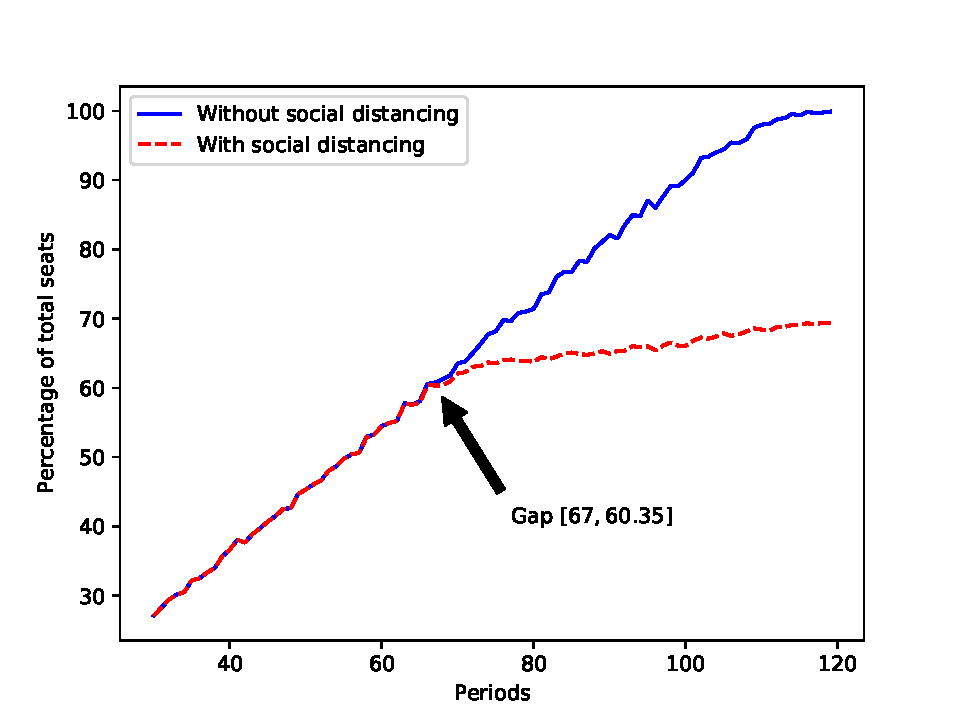
\includegraphics[width=0.48\textwidth]{./images/p2.pdf}}
          \end{figure}
        \scriptsize
        The gap point represents the first period where the number of people without social distancing is larger than that with social distancing and the gap percentage is the corresponding percentage of total seats.
    \end{frame}
      
    \begin{frame}{Estimation of Gap Point}
      \begin{figure}[ht]
        \centering
        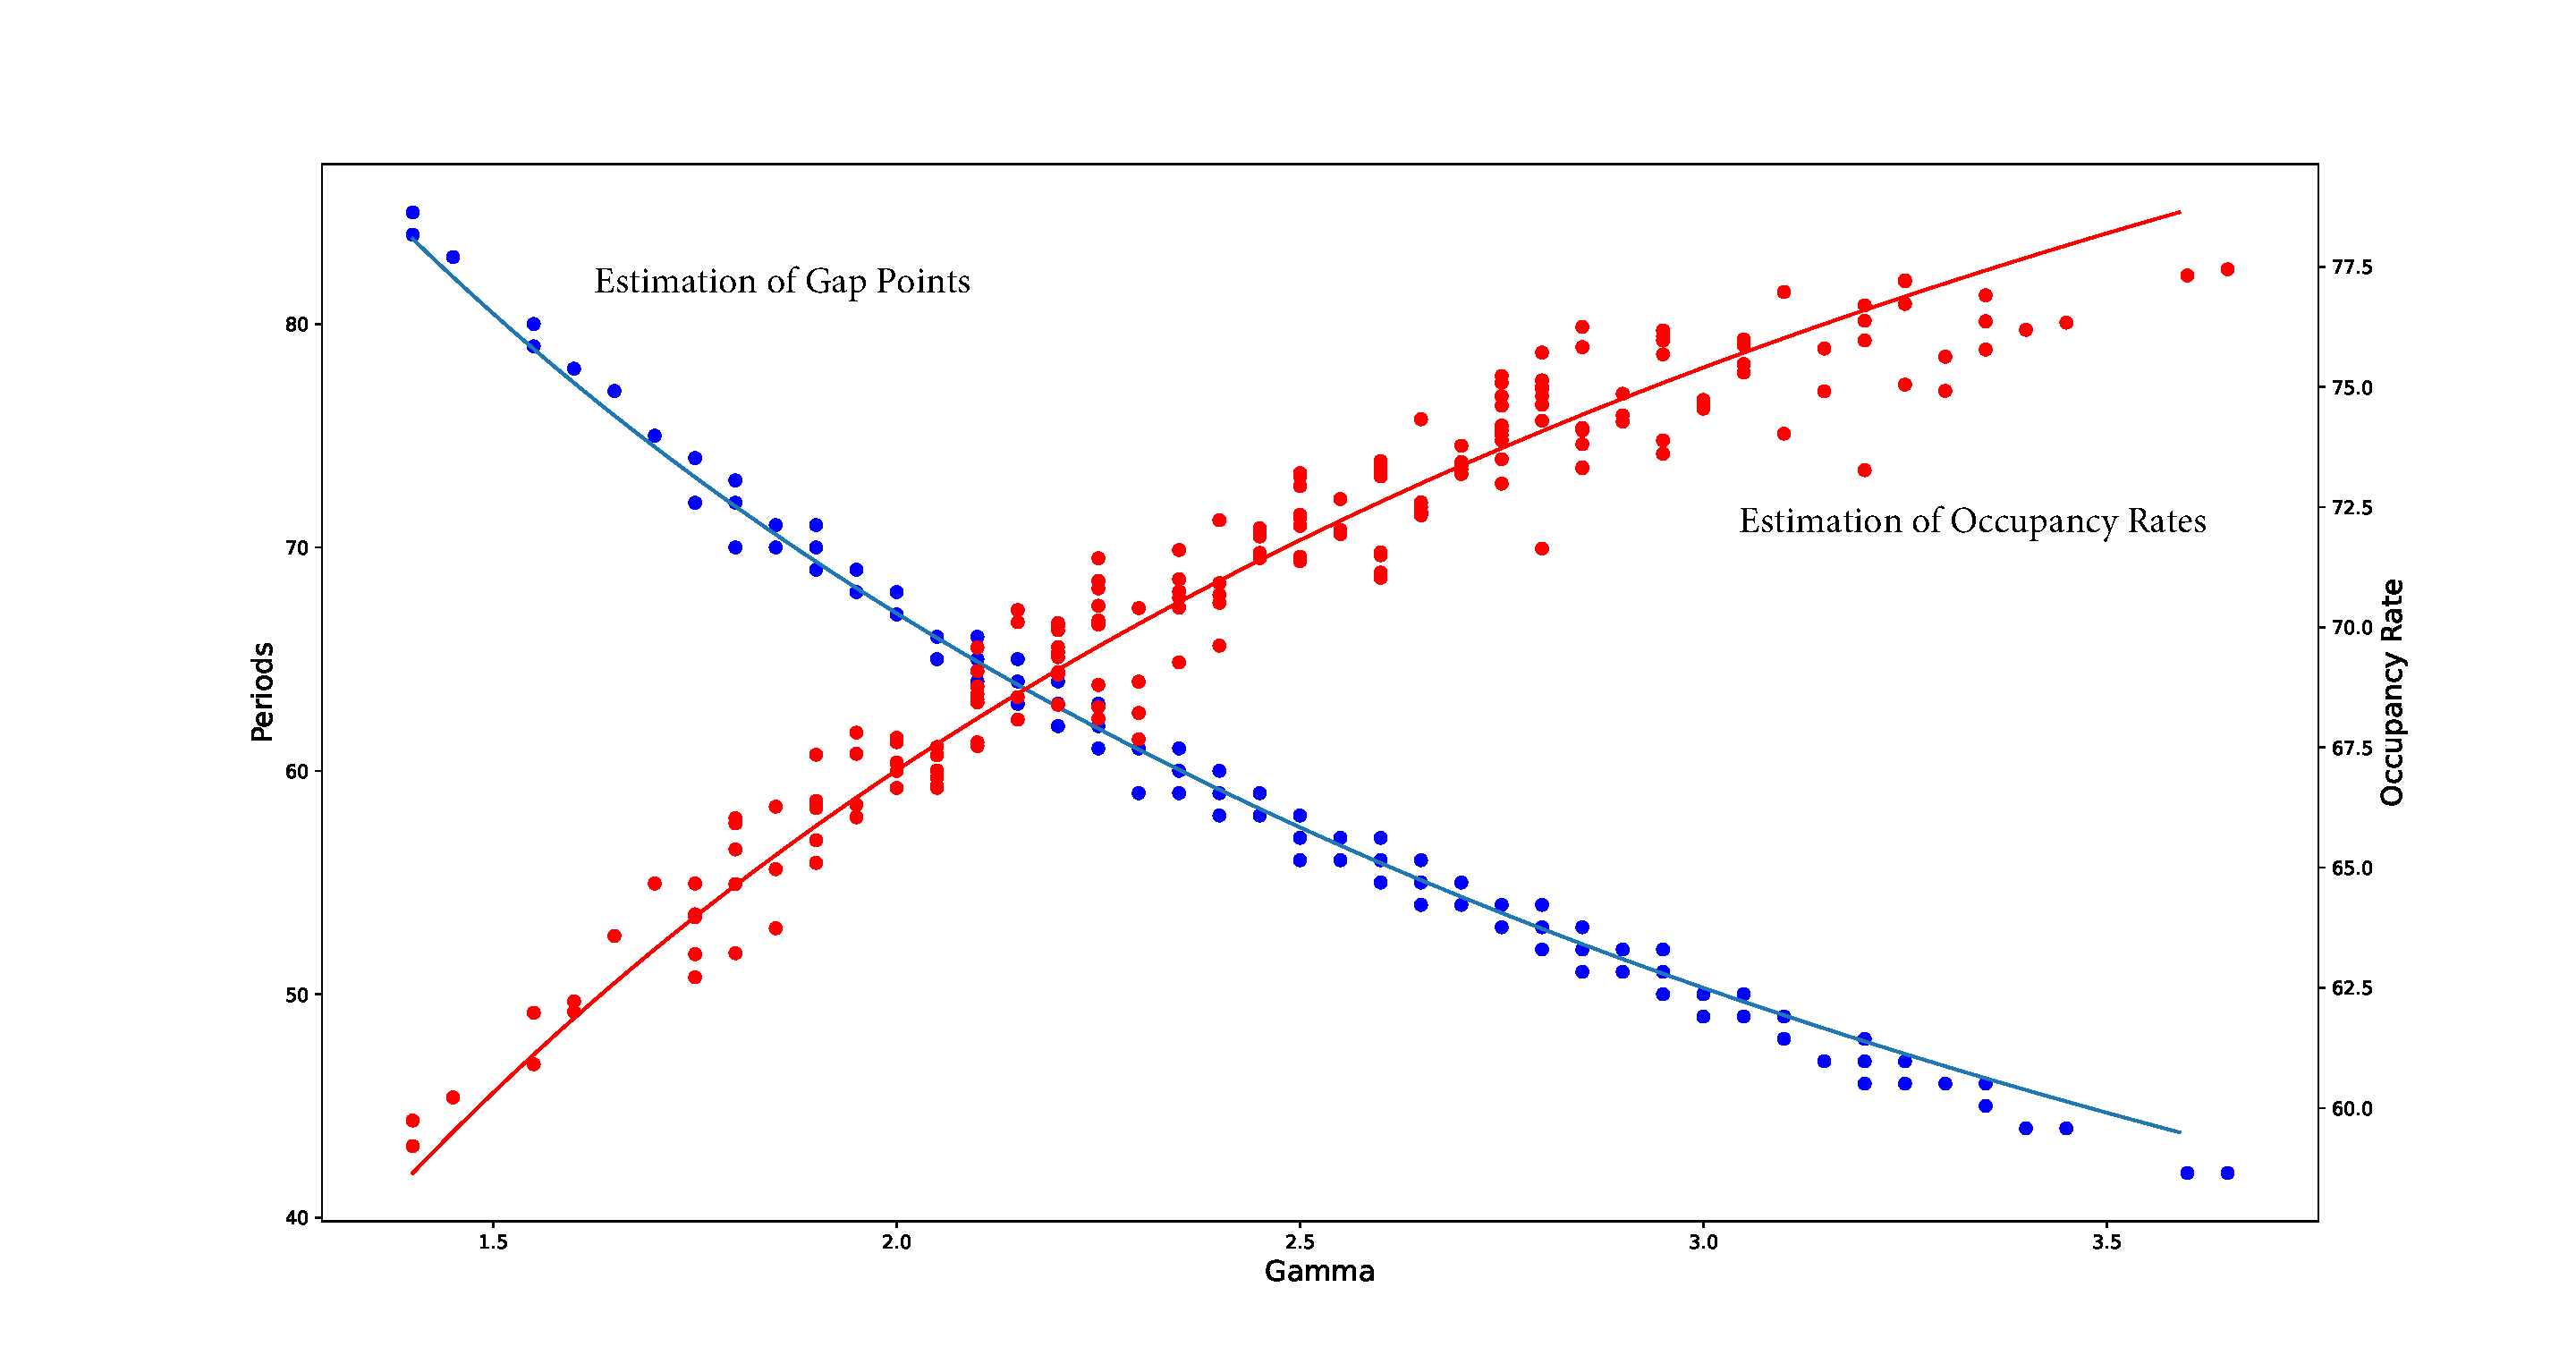
\includegraphics[width = 0.8\textwidth]{./images/gamma_estimation.pdf}
        \caption{Gap points with 200 probabilities}
    \end{figure}
    \scriptsize
    {\color{blue} Blue points}: period of the gap point.
    {\color{red} Red points}: occupancy rate of the gap point. 
    Gap points can be estimated.
    \end{frame}

    % We simulate 200 probabilities. For each probability, we run 100 instances to calculate the gap point and the corresponding occupancy rate. 
    
    % The point in the figure is the average of 100 instances. 
    % 


    \begin{frame}{Make A Later Allocation}
      This setting is particularly applicable to larger venues, such as stadiums, where an immediate decision is made when a group arrives, but the actual allocation of seats for that group is deferred to a later time.

      \vspace{0.5cm}

      The critical part is to make the decision, thus, we choose the following policies associated with relaxation forms.

      \vspace{0.5cm}

      Policies: 

      \begin{itemize}
        \item Dynamic programming based heuristic
        \item Bid-price control
      \end{itemize}
    \end{frame}

      \begin{frame}{Performances of Different Policies}
        \scriptsize
        \begin{table}[ht]
          \centering
          \begin{tabular}{|l|l|l|l|l|l|}
          \hline
           T & Probabilities &  DP1-L (\%) & Bid-L (\%) & DP1 (\%) & Bid (\%) \\
          \hline
          60  & [0.25, 0.25, 0.25, 0.25]  & 99.52 & 99.44 & 98.42 & 98.38 \\
          70  &   & 99.32 & 98.97 & 96.87 & 96.24 \\
          80  &   & 99.34 & 99.30 & 95.69 & 96.02 \\
          90  &   & 99.55 & 99.49 & 96.05 & 96.41  \\
          100 &   & 99.78 & 99.66 & 95.09 & 96.88 \\
          \hline
          60  & [0.25, 0.35, 0.05, 0.35]  & 99.50 & 99.37 & 98.26 & 98.25  \\
          70  &   & 99.40 & 98.97 & 96.62 & 96.06 \\
          80  &   & 99.46 & 99.24 & 96.01 & 95.89 \\
          90  &   & 99.59 & 99.35 & 96.77 & 96.62 \\
          100 &   & 99.77 & 99.61 & 97.04 & 97.14  \\
          \hline
          60  & [0.15, 0.25, 0.55, 0.05]  & 99.57 & 99.54 & 98.72 & 98.74 \\
          70  &   & 99.46 & 99.39  & 96.38 & 96.90 \\
          80  &   & 99.50 & 99.30  & 97.75 & 97.87 \\
          90  &   & 99.34 & 99.44  & 98.45 & 98.69 \\
          100 &   & 99.34 & 99.55  & 98.62 & 98.94 \\
          \hline
          \end{tabular}
        \end{table}

    \end{frame}

% !TEX root = sum1.tex
\section{Conclusion}
In conclusion, this paper addresses the problem of dynamic seat assignment with social distancing in the context of a pandemic. We propose a practical algorithm that balances seat utilization rates and the associated risk of infection to obtain a final seat planning that satisfies social distancing constraints when groups arrive. Our approach provides a comprehensive solution for optimizing seat assignments while ensuring the safety of customers. Our contributions include establishing a deterministic model to analyze the effects of social distancing when demand is known, using Benders decomposition methods to obtain the optimal solution for scenario-based stochastic programming, and developing a seat assignment policy for the dynamic situation. Our results demonstrate significant improvements over baseline strategies and provide guidance for developing attendance policies. Overall, our study highlights the importance of considering the operational significance behind social distancing and provides a new perspective for the government to adopt mechanisms for setting seat assignments to protect people in the post-pandemic era. Our study demonstrates the efficiency of obtaining the final seat planning using our proposed algorithm. The results indicate that our policy yields a seat planning that is very close to the optimal result. 

% Moreover, our analysis provides managerial guidance on how to set the occupancy rate and largest size of one group under the background of pandemic.


% \begin{table}[H]
%     \centering
%     \caption{xxxx}
%     \begin{tabular}{cccc}
%  \hline
%  a & aaaaaaaaa & aaaaaaaaaaaaaa & aaaaaaaaaaaaaaaaaaaa \\
%  \hline
%  a & \makebox[5ex][r]{123} & \makebox[6ex][r]{123456} & \makebox[6ex][r]{1}\\
%  a & \makebox[5ex][r]{12345} & \makebox[6ex][r]{123} & \makebox[6ex][r]{123} \\
%  a & \makebox[5ex][r]{1} & \makebox[6ex][r]{1234} & \makebox[6ex][r]{123456} \\
%  \hline
%  \end{tabular}
%  \end{table}

\bibliographystyle{plain}
\bibliography{refe}


% !TEX root = sum1.tex
\clearpage
\section*{Proof}

\begin{pf}[Theorem 1]
  \qed
\end{pf}

\begin{pf}[Lemma 1]
  \qed
\end{pf}

\begin{pf}[Lemma 2]
  \qed
\end{pf}

\begin{pf}[Theorem 2]
\qed
\end{pf}


\begin{pf}[Theorem 2]

\qed
\end{pf}

\begin{pf}[Theorem 3]

\qed
\end{pf}


\begin{pf}[Theorem 4]

\qed
\end{pf}

\begin{pf}[Theorem 5]

\qed
\end{pf}

\begin{pf}[Theorem 6]

\qed
\end{pf}

\begin{pf}[Lemma 2]

\qed
\end{pf}

\begin{pf}[Theorem 7]

\qed
\end{pf}

\begin{pf}[Lemma 4]

\qed
\end{pf}


\end{document}
